%! Author = zhiweizhang
%! Date = 10.06.25

\chapter{Results}\label{chapter:results}

\section{Evaluation Metrics}

To evaluate the performance of the classification models, we employ several standard metrics widely used in image
classification tasks. These metrics provide insight into the models' predictive capabilities across both binary and
multi-class scenarios.

Let:
\begin{itemize}
    \item $TP$ = True Positives
    \item $TN$ = True Negatives
    \item $FP$ = False Positives
    \item $FN$ = False Negatives
\end{itemize}

The evaluation metrics are defined as follows:

\begin{itemize}
  \item \textbf{Accuracy}:
  \begin{math}
  \text{Accuracy} = \frac{TP + TN}{TP + TN + FP + FN}
  \end{math}

  Accuracy provides an overall measure of how often the model is correct. It is most informative when class
  distributions are balanced.

  \item \textbf{Precision}:
  \begin{math}
  \text{Precision} = \frac{TP}{TP + FP}
  \end{math}

  Precision is particularly important when false positives carry a high cost.

  \item \textbf{Recall}:
  \begin{math}
  \text{Recall} = \frac{TP}{TP + FN}
  \end{math}

  Recall indicates the model’s ability to identify relevant instances, especially useful when false negatives are
  critical.

  \item \textbf{F1-Score}:
  \begin{math}
  \text{F1-Score} = 2 \times \frac{\text{Precision} \times \text{Recall}}{\text{Precision} + \text{Recall}}
  \end{math}

  F1-Score balances the trade-off between precision and recall and is useful when the class distribution is uneven.

  \item \textbf{Area Under the ROC Curve (AUC-ROC)}: AUC-ROC evaluates the model’s ability to distinguish between
  classes by plotting the True Positive Rate (TPR) against the False Positive Rate (FPR) at various thresholds.

  \begin{math}
  \text{TPR} = \frac{TP}{TP + FN}, \quad \text{FPR} = \frac{FP}{FP + TN}
  \end{math}
\end{itemize}

For multi-class classification, accuracy, precision, recall, and F1-score are computed using \textit{macro-averaging},
which calculates the metric independently for each class and then takes the average. This ensures equal treatment of
all classes, regardless of their frequency.

These metrics are reported for each model under both binary and multi-class classification settings. The
best-performing models were selected based on their validation loss, and the final results were obtained using the
corresponding test set.


\section{Binary Classification}
The binary classification result is showed as in ~\autoref{tab:binary-results},

%! Author = zhiweizhang
%! Date = 10.06.25

\begin{table}[ht]
\centering
\resizebox{\textwidth}{!}{
\begin{tabular}{lccccc}
\toprule
\textbf{Model}                        & \textbf{Accuracy} & \textbf{Precision} & \textbf{Recall} & \textbf{F1-Score} & \textbf{AUC}   \\
\midrule
YOLOv11                               & 0.995             & 0.793              & 0.932           & 0.857             & 0.964          \\
ResNet                                & 0.996             & 0.843              & 0.893           & 0.867             & 0.945          \\
EfficientNet                          & 0.993             & 0.772              & 0.761           & 0.767             & 0.878          \\
ViT                                   & 0.997             & 0.910              & 0.893           & 0.901             & 0.945          \\
Moondream                             & 0.718             & 0.046              & 1.000           & 0.088             & 0.857          \\
OpenCLIP                              & 0.314             & 0.013              & 0.639           & 0.025             & 0.474          \\
OpenCLIP + Logistic Regression        & 0.996             & 0.923              & 0.882           & 0.902             & 0.940          \\
OpenCLIP + SGDClassifier              & 0.996             & 0.924              & 0.880           & 0.901             & 0.939          \\
OpenCLIP + KNeighborsClassifier       & 0.996             & 0.895              & \textbf{0.936}  & 0.915             & \textbf{0.966} \\
OpenCLIP + SVC                        & \textbf{0.997}    & 0.948              & 0.929           & \textbf{0.939}    & 0.964          \\
OpenCLIP + DecisionTreeClassifier     & 0.987             & 0.674              & 0.742           & 0.706             & 0.867          \\
OpenCLIP + BaggingClassifier          & 0.989             & 0.744              & 0.717           & 0.730             & 0.856          \\
OpenCLIP + AdaBoostClassifier         & 0.994             & 0.901              & 0.791           & 0.842             & 0.894          \\
OpenCLIP + GradientBoostingClassifier & 0.993             & 0.879              & 0.801           & 0.838             & 0.899          \\
OpenCLIP + RandomForestClassifier     & 0.981             & \textbf{0.983}     & 0.097           & 0.177             & 0.548          \\
OpenCLIP + VotingClassifier           & 0.996             & 0.945              & 0.873           & 0.908             & 0.936          \\
\bottomrule
\end{tabular}
}
  \caption{Binary classification performance across different models. The best scores for each metric are highlighted in bold.}
\label{tab:binary-results}
\end{table}



\subsection{ROC and Precision-Recall Curves for Binary Classification}

To provide a more detailed view of model performance under imbalanced data conditions, we also plotted the Receiver
Operating Characteristic (ROC) curve and Precision-Recall (PR) curve for the binary classification task. These
curves allow for a better understanding of how each model balances sensitivity and specificity across different
thresholds.

~\autoref{fig:roc-curve} displays the ROC curves, highlighting the trade-off between true positive rate (TPR) and
false positive rate (FPR). AUC scores (reported in ~\autoref{tab:binary-results}) align with the visual performance
in this plot.

~\autoref{fig:pr-curve} shows the PR curves, which are especially informative for evaluating classifier
performance under class imbalance. The area under the PR curve (average precision) complements the ROC AUC and
emphasizes how well models perform in retrieving relevant positive samples.

\begin{figure}[ht]
  \centering
  
\includegraphics[width=0.8\textwidth]{ROC}
  \caption{ROC curves of all models on the binary classification task.}
  \label{fig:roc-curve}
\end{figure}

\begin{figure}[ht]
  \centering
  
\includegraphics[width=0.8\textwidth]{PR}
  \caption{Precision-Recall curves of all models on the binary classification task.}
  \label{fig:pr-curve}
\end{figure}

\subsubsection{Reduced-Symbol Set Experiment}
To further evaluate the robustness of our models, we conducted an additional experiment using a reduced nazi symbol set from the
original dataset. This set included only the three most visually distinct symbols, specifically ss skull, siegrune, and Swastika.
The results of this experiment are shown in ~\autoref{tab:binary-reduced-symbols-result}.

%! Author = zhiweizhang
%! Date = 10.06.25

\begin{table}[ht]
  \centering
  \resizebox{\textwidth}{!}{
    \begin{tabular}{lccccc}
    \toprule
    \textbf{Model}                        & \textbf{Accuracy} & \textbf{Precision} & \textbf{Recall} & \textbf{F1-Score} & \textbf{AUC}   \\
    \midrule
    YOLOv11                               & 0.994             & 0.792              & 0.568           & 0.661             & 0.783          \\
    ResNet                                & 0.994             & 0.712              & 0.750           & 0.730             & 0.873          \\
    EfficientNet                          & 0.988             & 0.781              & 0.558           & 0.651             & 0.777          \\
    ViT                                   & \textbf{0.998}    & 0.972              & 0.926           & \textbf{0.948}    & 0.962          \\
    Moondream                             & 0.996             & 0.840              & 0.851           & 0.846             & 0.924          \\
    OpenCLIP                              & 0.864             & 0.025              & 0.338           & 0.047             & 0.604          \\
    OpenCLIP + Logistic Regression        & 0.996             & 0.917              & 0.835           & 0.874             & 0.917          \\
    OpenCLIP + SGDClassifier              & 0.996             & 0.899              & 0.895           & 0.897             & 0.946          \\
    OpenCLIP + KNeighborsClassifier       & \textbf{0.998}    & 0.895              & \textbf{0.989}  & 0.940             & \textbf{0.993} \\
    OpenCLIP + SVC                        & \textbf{0.998}    & \textbf{0.973}     & 0.900           & 0.935             & 0.949          \\
    OpenCLIP + DecisionTreeClassifier     & 0.985             & 0.514              & 0.635           & 0.568             & 0.812          \\
    OpenCLIP + BaggingClassifier          & 0.987             & 0.566              & 0.639           & 0.600             & 0.815          \\
    OpenCLIP + AdaBoostClassifier         & 0.994             & 0.869              & 0.742           & 0.800             & 0.869          \\
    OpenCLIP + GradientBoostingClassifier & 0.993             & 0.837              & 0.708           & 0.767             & 0.853          \\
    OpenCLIP + RandomForestClassifier     & 0.988             & 0.959              & 0.209           & 0.344             & 0.604          \\
    OpenCLIP + VotingClassifier           & 0.997             & 0.964              & 0.833           & 0.894             & 0.916          \\
    \bottomrule
    \end{tabular}
  }
  \caption{Binary classification performance across different models on reduced-symbol set. The best scores for each metric are highlighted in bold.}
  \label{tab:binary-reduced-symbols-result}
\end{table}

\subsection{Multi-class Classification}

The muilti-class classification result is showed as in ~\autoref{tab:multi-class-results},

%! Author = zhiweizhang
%! Date = 10.06.25

\begin{table}[ht]
\centering
\resizebox{\textwidth}{!}{
\begin{tabular}{lcccc}
\toprule
\textbf{Model}                        & \textbf{Accuracy (Macro)} & \textbf{Precision (Macro)} & \textbf{Recall (Macro)} & \textbf{F1-score (Macro)} \\
\midrule
YOLOv11                               & \textbf{0.884}            & \textbf{0.865}             & \textbf{0.818}          & \textbf{0.833}            \\
ResNet                                & 0.879                     & 0.850                      & 0.795                   & 0.810                     \\
EfficientNet                          & 0.794                     & 0.710                      & 0.697                   & 0.698                     \\
ViT                                   & 0.876                     & 0.833                      & 0.775                   & 0.790                     \\
Moondream                             & 0.608                     & 0.412                      & 0.601                   & 0.355                     \\
OpenCLIP                              & 0.274                     & 0.354                      & 0.413                   & 0.265                     \\
OpenCLIP + Logistic Regression        & 0.768                     & 0.476                      & 0.390                   & 0.412                     \\
OpenCLIP + SGDClassifier              & 0.799                     & 0.749                      & 0.624                   & 0.632                     \\
OpenCLIP + KNeighborsClassifier       & 0.752                     & 0.598                      & 0.518                   & 0.530                     \\
OpenCLIP + SVC                        & 0.815                     & 0.723                      & 0.593                   & 0.620                     \\
OpenCLIP + DecisionTreeClassifier     & 0.577                     & 0.177                      & 0.160                   & 0.154                     \\
OpenCLIP + BaggingClassifier          & 0.599                     & 0.320                      & 0.179                   & 0.177                     \\
OpenCLIP + AdaBoostClassifier         & 0.648                     & 0.404                      & 0.275                   & 0.305                     \\
OpenCLIP + GradientBoostingClassifier & 0.704                     & 0.444                      & 0.412                   & 0.389                     \\
OpenCLIP + RandomForestClassifier     & 0.583                     & 0.261                      & 0.162                   & 0.161                     \\
OpenCLIP + VotingClassifier           & 0.770                     & 0.481                      & 0.391                   & 0.415                     \\
\bottomrule
\end{tabular}
}
  \caption{Multi-class classification performance across different models. The best scores for each metric are highlighted in bold.}
\label{tab:multi-class-results}
\end{table}

\subsection{Comparison of Evaluation Metrics Across Models}

To provide a comprehensive visual overview of model performance across different evaluation criteria, we present bar
plots comparing all selected models (YOLOv11, ResNet50, EfficientNet-B2, ViT, Moondream, OpenCLIP, OpenCLIP + SVC)
under both binary and multi-class classification settings.

~\autoref{fig:model-accuracy}, \autoref{fig:model-precision}, \autoref{fig:model-recall}, and
~\autoref{fig:model-f1-score} show side-by-side comparisons of accuracy,
precision, recall, and F1-score respectively. These visualizations make it easier to observe performance trade-offs
between models and help identify consistently strong performers across metrics.

Overall, YOLOv11 and OpenCLIP-based models exhibit the highest performance across most metrics, particularly in
binary classification tasks. In contrast, models like Moondream and EfficientNet-B2 show lower consistency,
especially in multi-class classification. These observations suggest that embedding-based and detection-based
methods may generalize better across symbol types.



%! Author = zhiweizhang
%! Date = 11.06.25

% Preamble
\begin{figure}[ht]
    \centering
    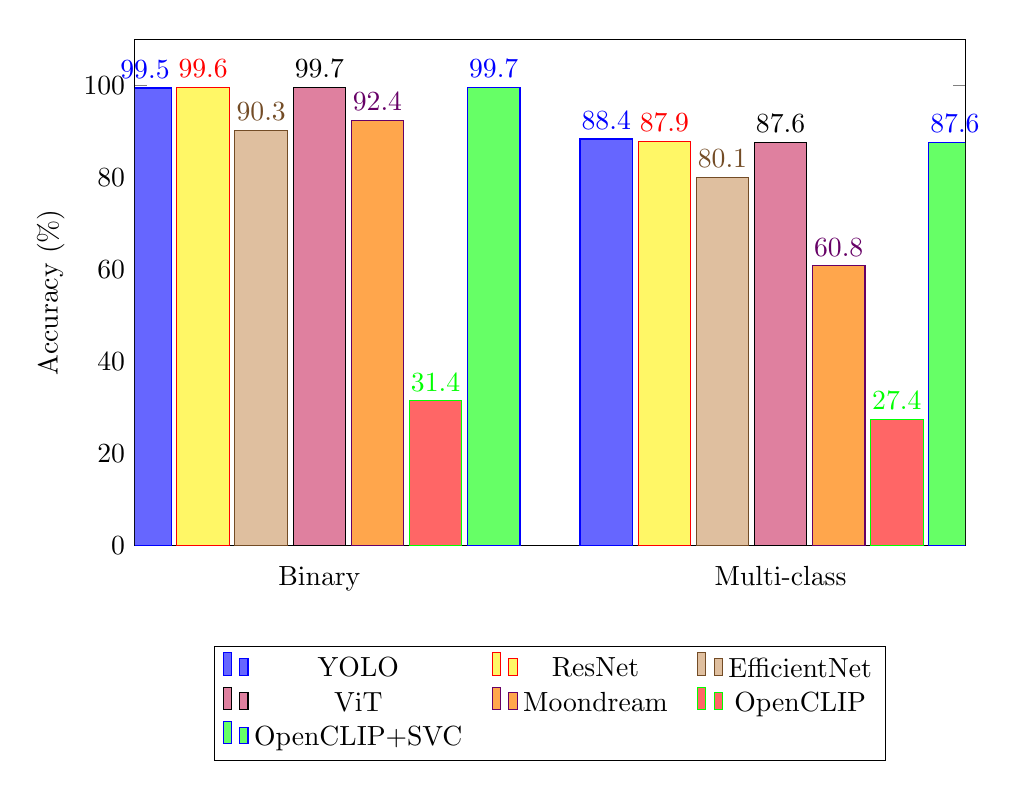
\begin{tikzpicture}
        \begin{axis}[
            ybar,
            bar width=19pt,
            width=\textwidth,
            height=8cm,
            enlarge x limits=0.4,
            ylabel={Accuracy (\%)},
            symbolic x coords={Binary, Multi-class},
            xtick=data,
            ymin=0.0, ymax=110.0,
            nodes near coords,
            nodes near coords align={vertical},
            major x tick style = transparent,
            legend style={
                at={(0.5,-0.2)},
                anchor=north,
                legend columns=3,
                /tikz/every even column/.append style={column sep=0.3cm}
            }
        ]
        \addplot+[style={fill=blue!60}]      coordinates {(Binary, 99.5) (Multi-class, 88.4)};
        \addplot+[style={fill=yellow!60}]    coordinates {(Binary, 99.6) (Multi-class, 87.9)};
        \addplot+[style={fill=brown!50}]     coordinates {(Binary, 90.3) (Multi-class, 80.1)};
        \addplot+[style={fill=purple!50}]    coordinates {(Binary, 99.7) (Multi-class, 87.6)};
        \addplot+[style={fill=orange!70}]    coordinates {(Binary, 92.4) (Multi-class, 60.8)};
        \addplot+[style={fill=red!60}]       coordinates {(Binary, 31.4) (Multi-class, 27.4)};
        \addplot+[style={fill=green!60}]     coordinates {(Binary, 99.7) (Multi-class, 87.6)};
        \legend{
            YOLO,
            ResNet,
            EfficientNet,
            ViT,
            Moondream,
            OpenCLIP,
            OpenCLIP+SVC
        }
        \end{axis}
    \end{tikzpicture}
    \caption{Comparison of accuracy scores for all models on binary (left) and multi-class (right) classification tasks.}
    \label{fig:model-accuracy}
\end{figure}
%! Author = zhiweizhang
%! Date = 11.06.25

% Preamble
\begin{figure}[ht]
    \centering
    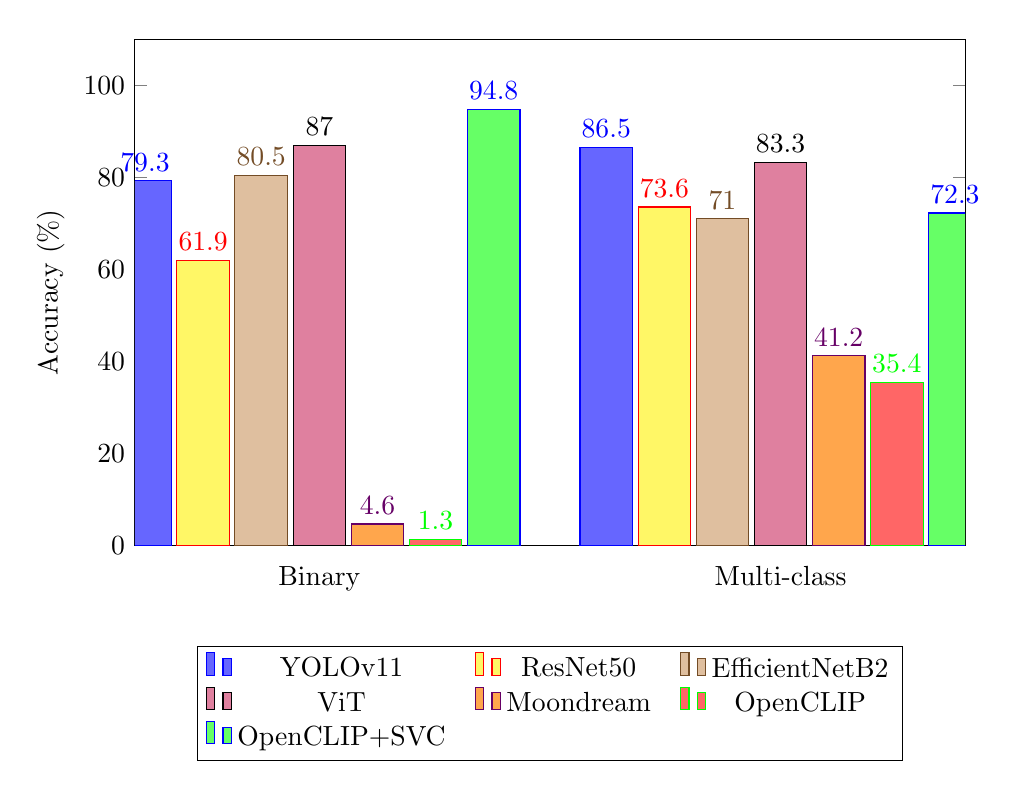
\begin{tikzpicture}
        \begin{axis}[
            ybar,
            bar width=19pt,
            width=\textwidth,
            height=8cm,
            enlarge x limits=0.4,
            ylabel={Accuracy (\%)},
            symbolic x coords={Binary, Multi-class},
            xtick=data,
            ymin=0.0, ymax=110.0,
            nodes near coords,
            nodes near coords align={vertical},
            major x tick style = transparent,
            legend style={
                at={(0.5,-0.2)},
                anchor=north,
                legend columns=3,
                /tikz/every even column/.append style={column sep=0.3cm}
            }
        ]
        \addplot+[style={fill=blue!60}]      coordinates {(Binary, 79.3) (Multi-class, 86.5)};
        \addplot+[style={fill=yellow!60}]    coordinates {(Binary, 61.9) (Multi-class, 73.6)};
        \addplot+[style={fill=brown!50}]     coordinates {(Binary, 80.5) (Multi-class, 71.0)};
        \addplot+[style={fill=purple!50}]    coordinates {(Binary, 87.0) (Multi-class, 83.3)};
        \addplot+[style={fill=orange!70}]    coordinates {(Binary, 4.6) (Multi-class, 41.2)};
        \addplot+[style={fill=red!60}]       coordinates {(Binary, 1.3) (Multi-class, 35.4)};
        \addplot+[style={fill=green!60}]     coordinates {(Binary, 94.8) (Multi-class, 72.3)};
        \legend{
            YOLOv11,
            ResNet50,
            EfficientNetB2,
            ViT,
            Moondream,
            OpenCLIP,
            OpenCLIP+SVC
        }
        \end{axis}
    \end{tikzpicture}
    \caption{Classification precision of selected models for binary and multi-class tasks.}
    \label{fig:model-precision}
\end{figure}
%! Author = zhiweizhang
%! Date = 11.06.25

% Preamble
\begin{figure}[ht]
    \centering
    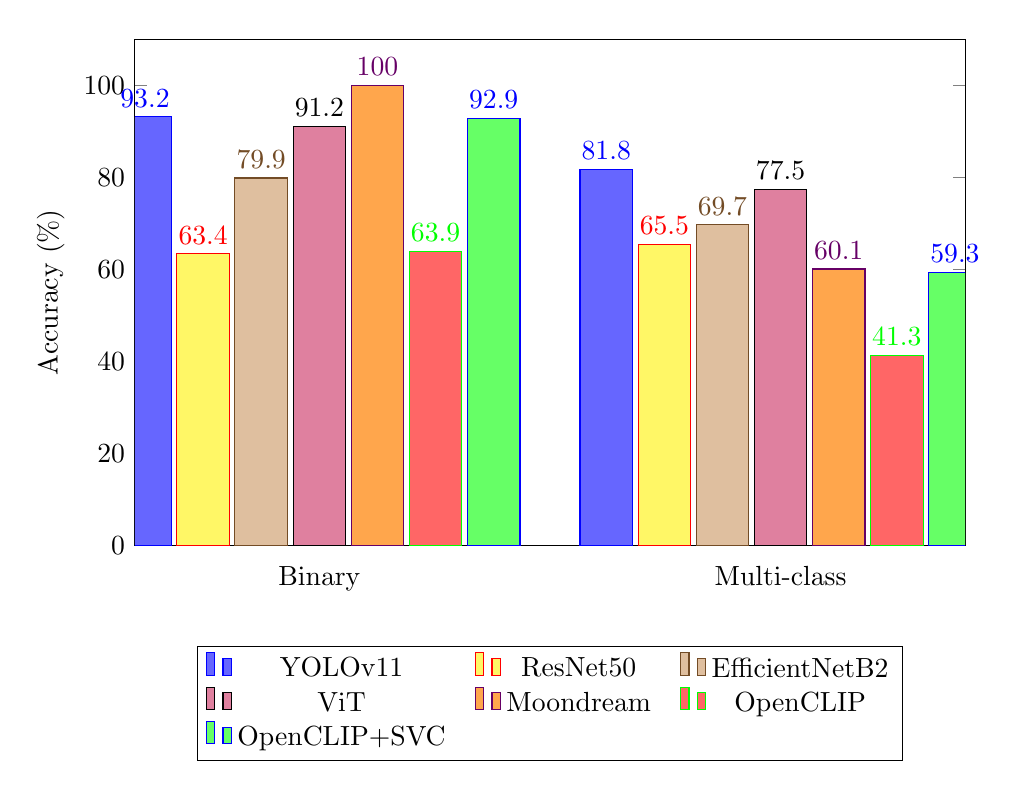
\begin{tikzpicture}
        \begin{axis}[
            ybar,
            bar width=19pt,
            width=\textwidth,
            height=8cm,
            enlarge x limits=0.4,
            ylabel={Accuracy (\%)},
            symbolic x coords={Binary, Multi-class},
            xtick=data,
            ymin=0.0, ymax=110.0,
            nodes near coords,
            nodes near coords align={vertical},
            major x tick style = transparent,
            legend style={
                at={(0.5,-0.2)},
                anchor=north,
                legend columns=3,
                /tikz/every even column/.append style={column sep=0.3cm}
            }
        ]
        \addplot+[style={fill=blue!60}]      coordinates {(Binary, 93.2) (Multi-class, 81.8)};
        \addplot+[style={fill=yellow!60}]    coordinates {(Binary, 63.4) (Multi-class, 65.5)};
        \addplot+[style={fill=brown!50}]     coordinates {(Binary, 79.9) (Multi-class, 69.7)};
        \addplot+[style={fill=purple!50}]    coordinates {(Binary, 91.2) (Multi-class, 77.5)};
        \addplot+[style={fill=orange!70}]    coordinates {(Binary, 100.0) (Multi-class, 60.1)};
        \addplot+[style={fill=red!60}]       coordinates {(Binary, 63.9) (Multi-class, 41.3)};
        \addplot+[style={fill=green!60}]     coordinates {(Binary, 92.9) (Multi-class, 59.3)};
        \legend{
            YOLOv11,
            ResNet50,
            EfficientNetB2,
            ViT,
            Moondream,
            OpenCLIP,
            OpenCLIP+SVC
        }
        \end{axis}
    \end{tikzpicture}
    \caption{Comparison of recall scores for all models on binary (left) and multi-class (right) classification tasks.}
    \label{fig:model-recall}
\end{figure}
%! Author = zhiweizhang
%! Date = 11.06.25

% Preamble
\begin{figure}[ht]
    \centering
    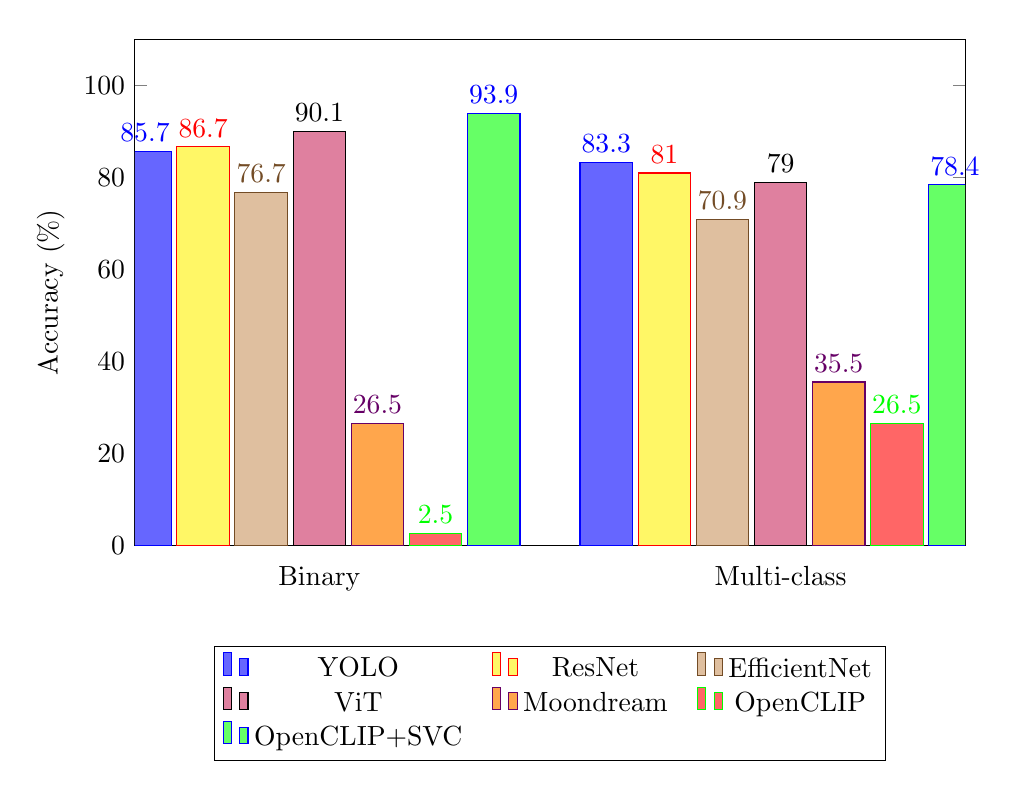
\begin{tikzpicture}
        \begin{axis}[
            ybar,
            bar width=19pt,
            width=\textwidth,
            height=8cm,
            enlarge x limits=0.4,
            ylabel={Accuracy (\%)},
            symbolic x coords={Binary, Multi-class},
            xtick=data,
            ymin=0.0, ymax=110.0,
            nodes near coords,
            nodes near coords align={vertical},
            major x tick style = transparent,
            legend style={
                at={(0.5,-0.2)},
                anchor=north,
                legend columns=3,
                /tikz/every even column/.append style={column sep=0.3cm}
            }
        ]
        \addplot+[style={fill=blue!60}]      coordinates {(Binary, 85.7) (Multi-class, 83.3)};
        \addplot+[style={fill=yellow!60}]    coordinates {(Binary, 86.7) (Multi-class, 81.0)};
        \addplot+[style={fill=brown!50}]     coordinates {(Binary, 76.7) (Multi-class, 70.9)};
        \addplot+[style={fill=purple!50}]    coordinates {(Binary, 90.1) (Multi-class, 79.0)};
        \addplot+[style={fill=orange!70}]    coordinates {(Binary, 26.5) (Multi-class, 35.5)};
        \addplot+[style={fill=red!60}]       coordinates {(Binary, 2.5) (Multi-class, 26.5)};
        \addplot+[style={fill=green!60}]     coordinates {(Binary, 93.9) (Multi-class, 78.4)};
        \legend{
            YOLO,
            ResNet,
            EfficientNet,
            ViT,
            Moondream,
            OpenCLIP,
            OpenCLIP+SVC
        }
        \end{axis}
    \end{tikzpicture}
    \caption{Comparison of F1-score values for all models on binary (left) and multi-class (right) classification tasks.}
    \label{fig:model-f1-score}
\end{figure}